%auto-ignore
\documentclass{standalone}

\usepackage{graphicx}
\usepackage{tikz}

\begin{document}
\begin{tikzpicture}
\node[inner sep=0pt,align=center,label={[yshift=0.50cm]\textbf{prepare} \#1}]
(proc1) at (0,0)
	{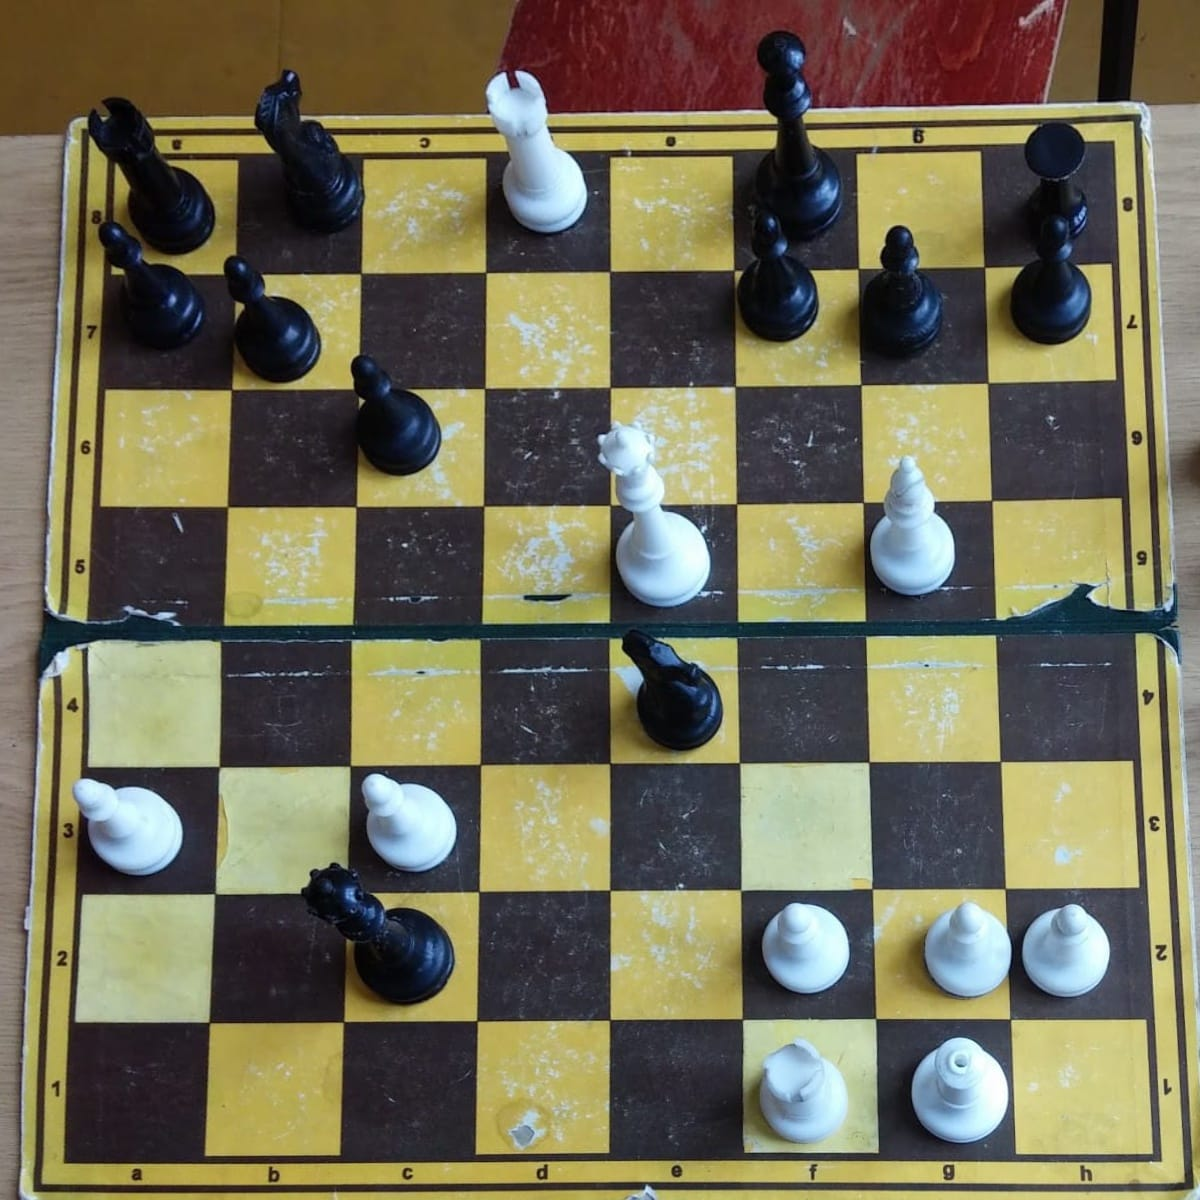
\includegraphics[width=.25\textwidth]{figure3_1a.jpg}\\[1em]
	 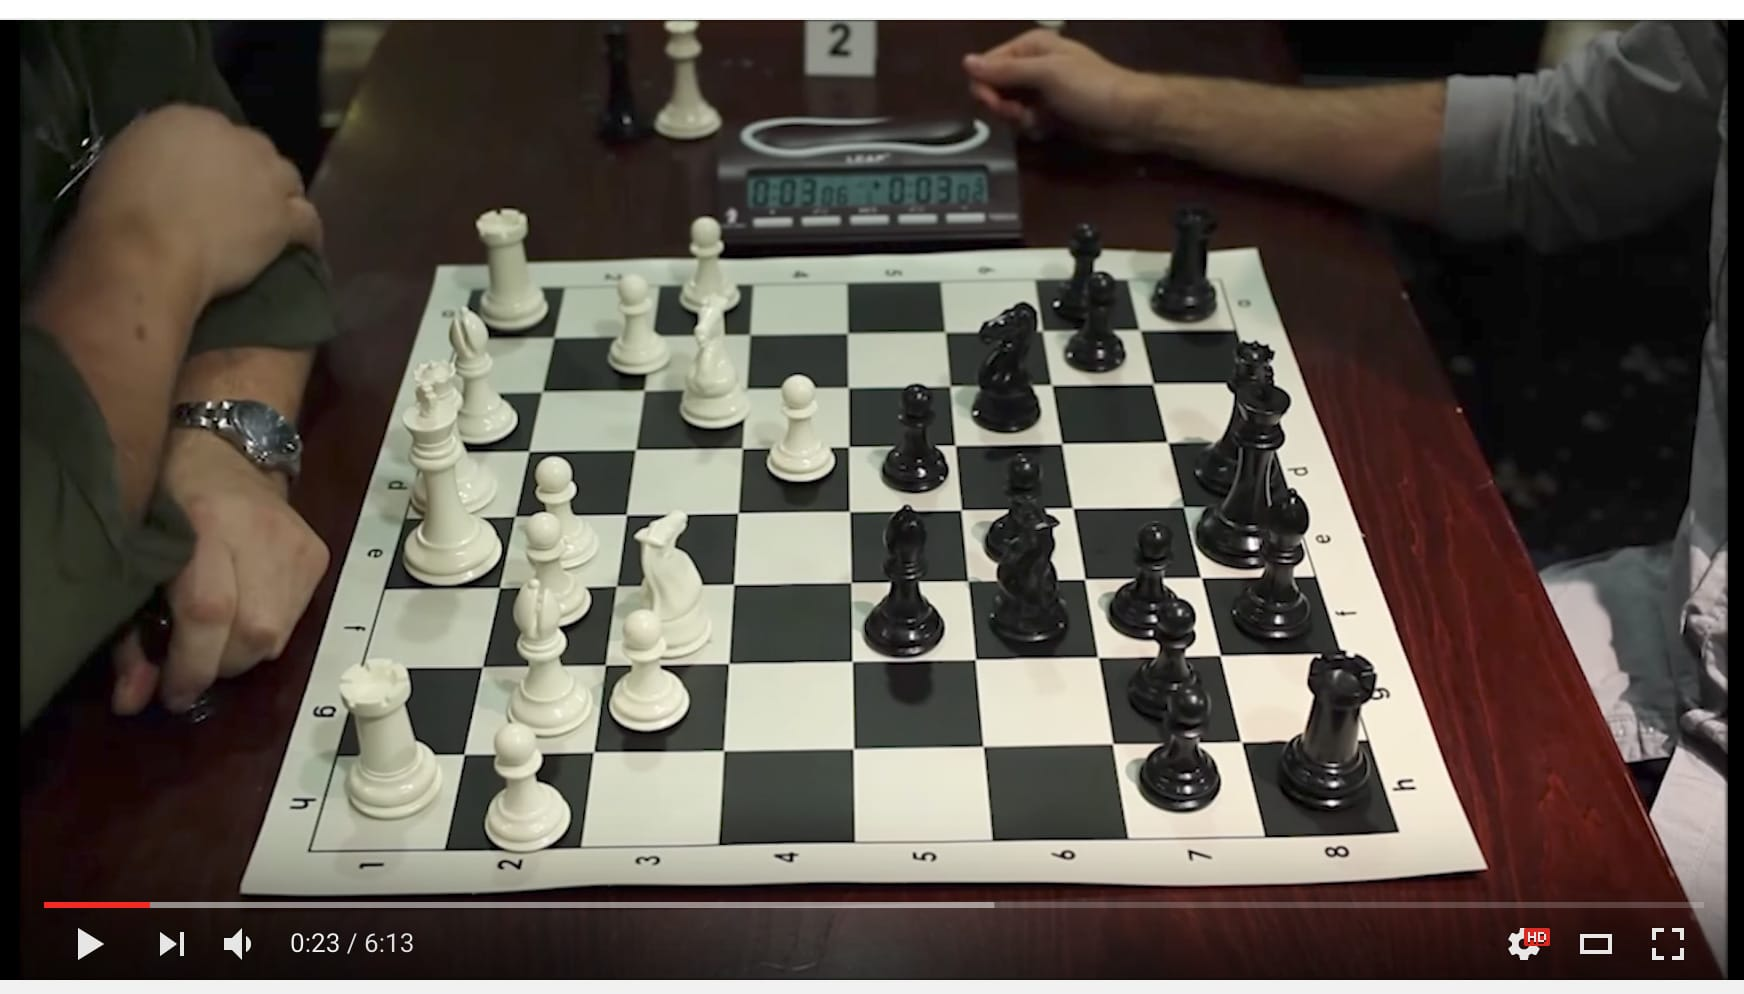
\includegraphics[width=.25\textwidth]{figure3_1b.jpg}\\[1em]
	 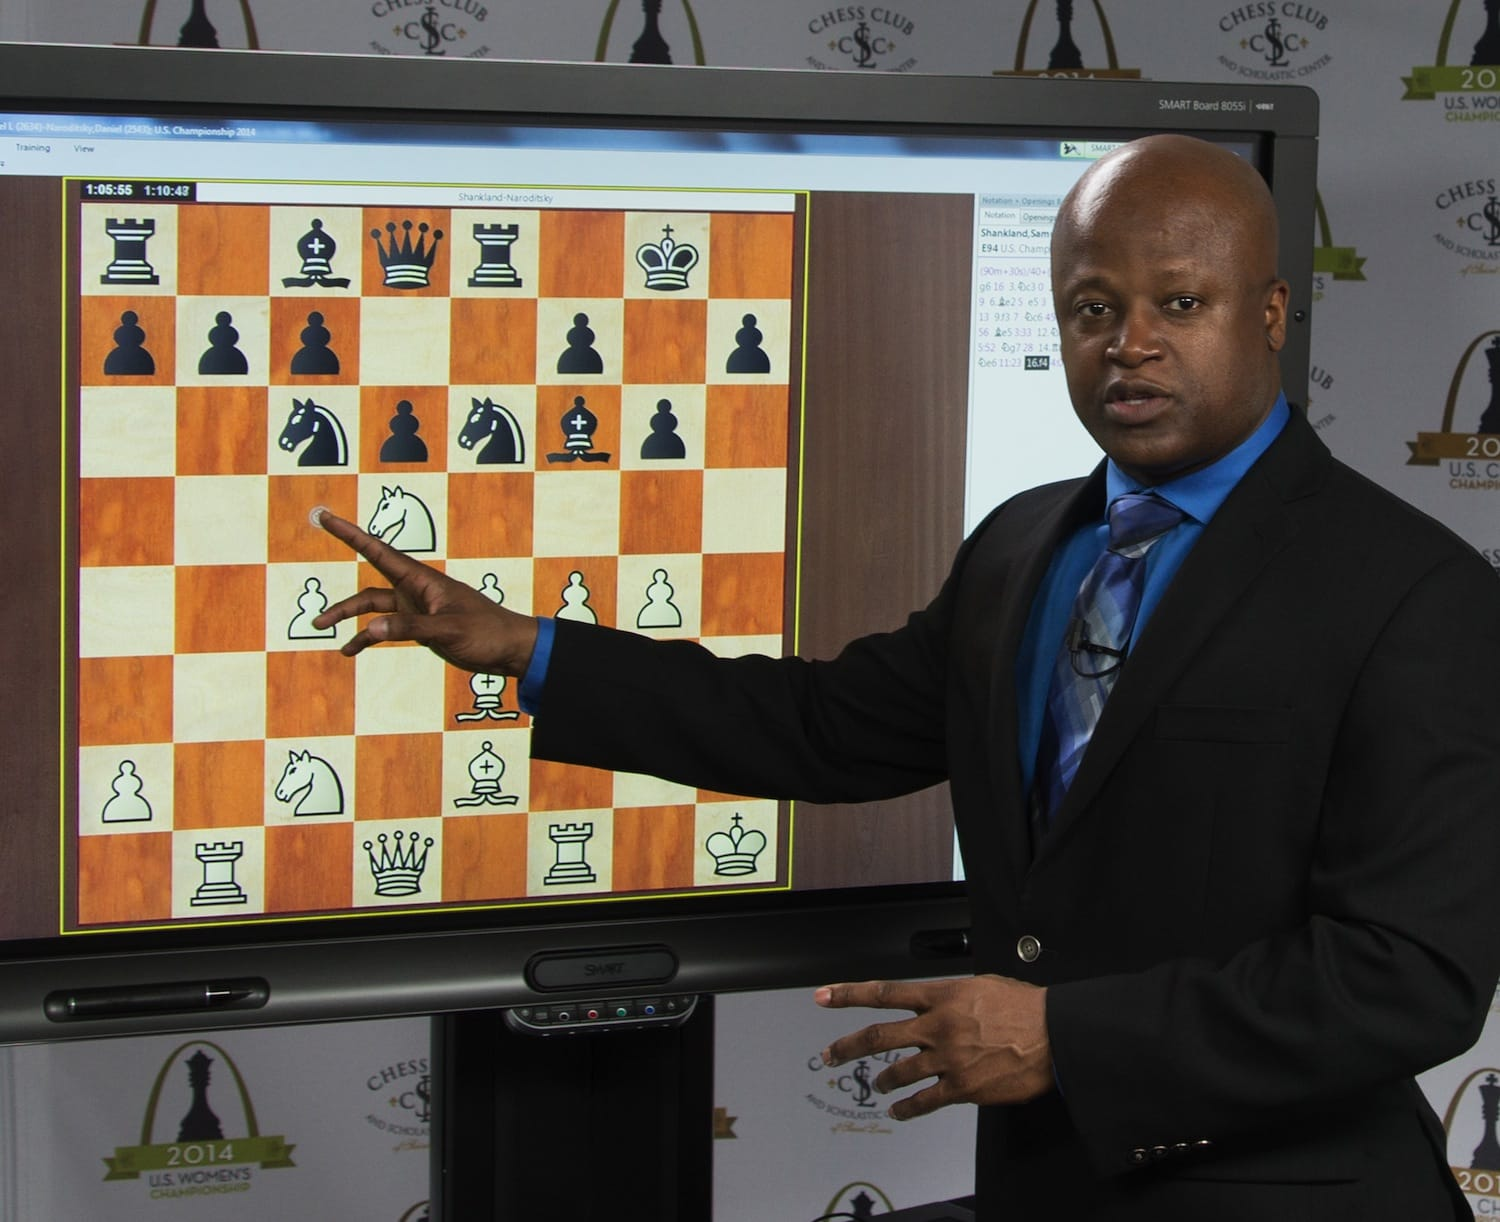
\includegraphics[width=.25\textwidth]{figure3_1c.jpg}};
\node[inner sep=0pt,align=center,label={[yshift=0.50cm]\textbf{FAPL} \#2}]
(proc2) at (6,0)
	{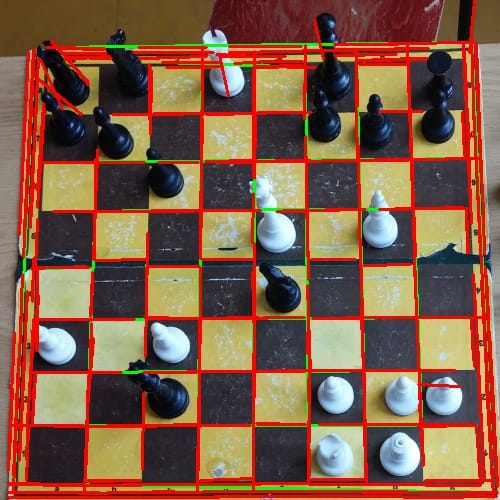
\includegraphics[width=.25\textwidth]{figure3_2a.jpg}\\[1em]
	 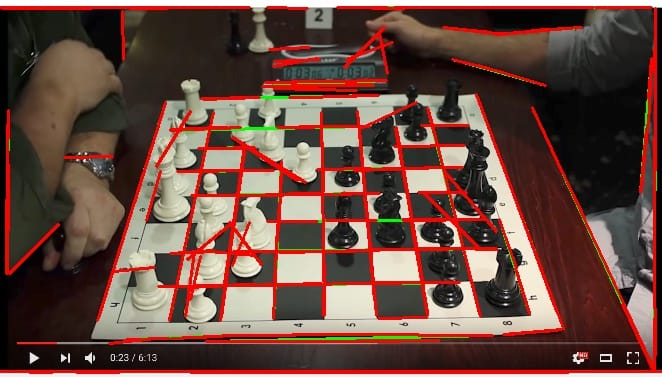
\includegraphics[width=.25\textwidth]{figure3_2b.jpg}\\[1em]
	 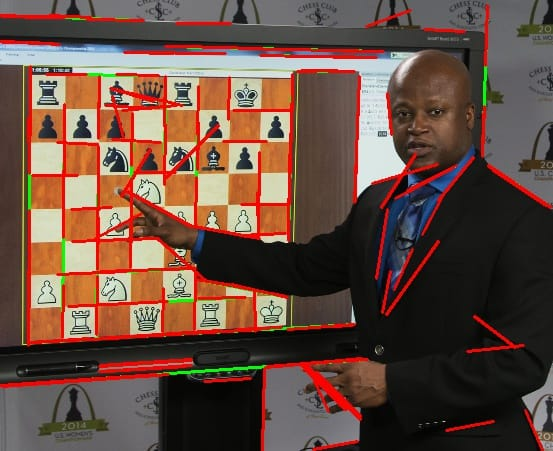
\includegraphics[width=.25\textwidth]{figure3_2c.jpg}};
\node[inner sep=0pt,align=center,label={[yshift=0.50cm]\textbf{PAMG} \#3}]
(proc3) at (12,0)
	{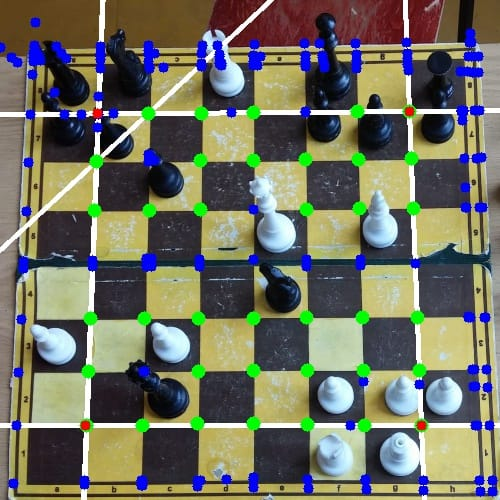
\includegraphics[width=.25\textwidth]{figure3_3a.jpg}\\[1em]
	 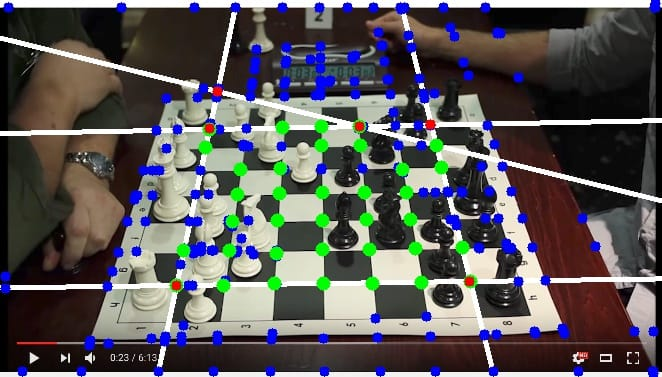
\includegraphics[width=.25\textwidth]{figure3_3b.jpg}\\[1em]
	 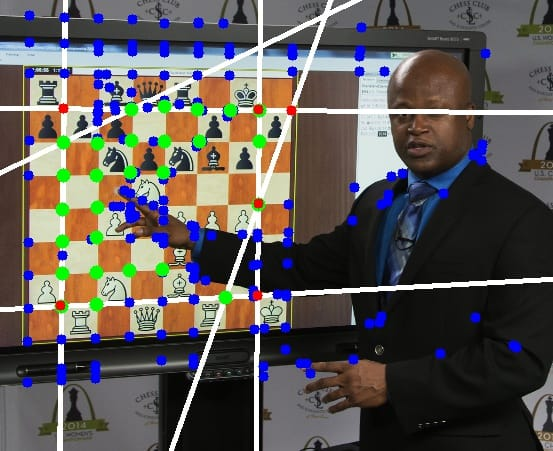
\includegraphics[width=.25\textwidth]{figure3_3c.jpg}};
\node[inner sep=0pt,align=center,label={[yshift=0.50cm]\textbf{reconstruct} \#4}]
(proc4) at (18,0)
	{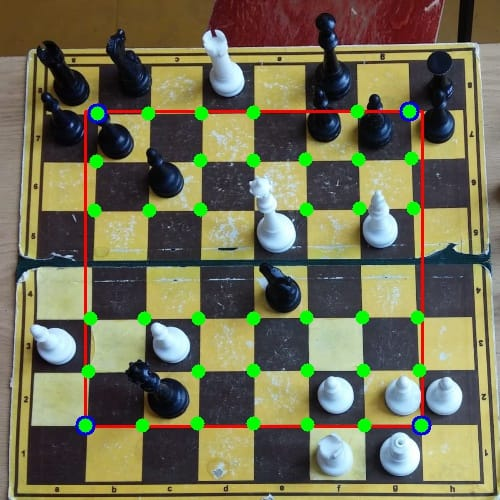
\includegraphics[width=.25\textwidth]{figure3_4a.jpg}\\[1em]
	 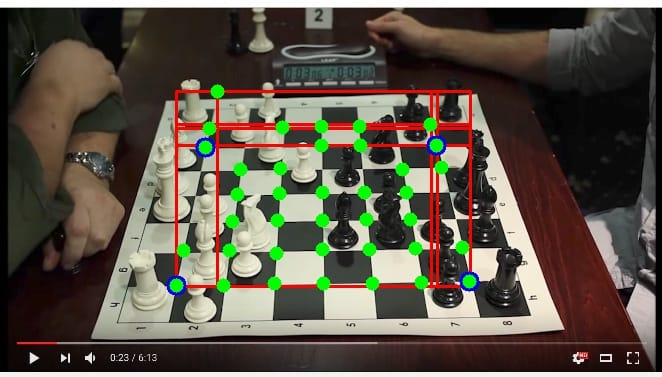
\includegraphics[width=.25\textwidth]{figure3_4b.jpg}\\[1em]
	 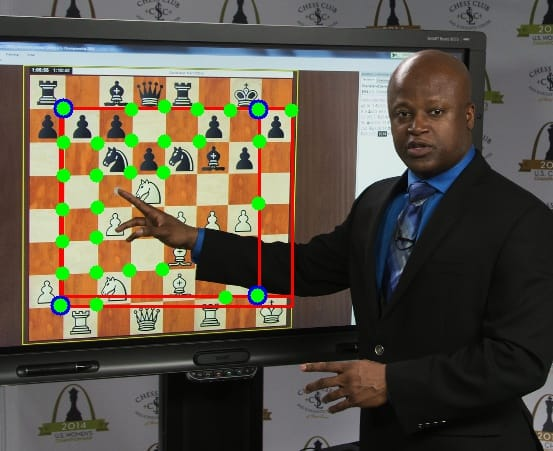
\includegraphics[width=.25\textwidth]{figure3_4c.jpg}};
\node[inner sep=0pt,align=center,label={[yshift=0.50cm]\textbf{crop} \#5}]
(proc5) at (24,0)
	{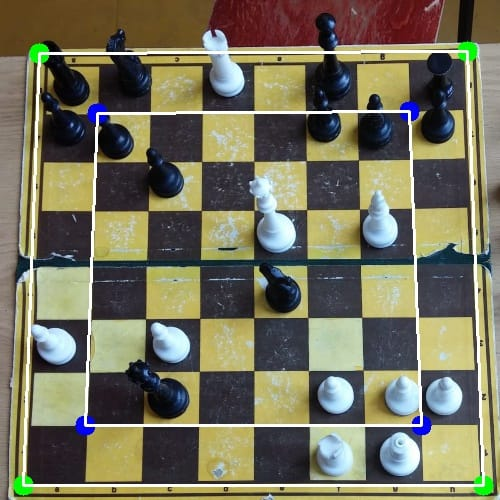
\includegraphics[width=.25\textwidth]{figure3_5a.jpg}\\[1em]
	 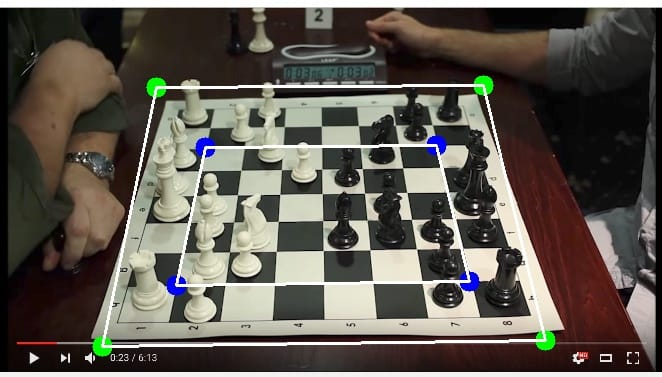
\includegraphics[width=.25\textwidth]{figure3_5b.jpg}\\[1em]
	 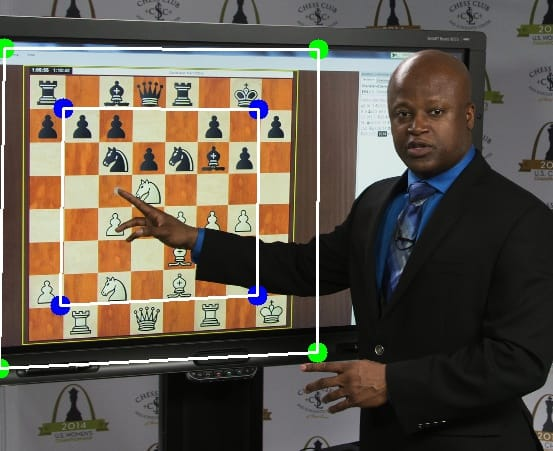
\includegraphics[width=.25\textwidth]{figure3_5c.jpg}};
\draw[->,thick,shorten >=6pt,shorten <=6pt] (proc1) -- (proc2)
	node[midway,fill=white,align=center,rotate=90,anchor=north,yshift=0.8cm]
	{\huge find\\interesting\\lines};
\draw[->,thick,shorten >=6pt,shorten <=6pt] (proc2) -- (proc3)
	node[midway,fill=white,align=center,rotate=90,anchor=north,yshift=0.6cm]
	{\huge analyze\\intersections};
\draw[->,thick,shorten >=6pt,shorten <=6pt] (proc3) -- (proc4)
	node[midway,fill=white,align=center,rotate=90,anchor=north,yshift=0.8cm]
	{\huge adjust\\mesh\\grid};
\draw[->,thick,shorten >=6pt,shorten <=6pt] (proc4) -- (proc5)
	node[midway,fill=white,align=center,rotate=90,anchor=north,yshift=0.8cm]
	{\huge padcrop\\next\\layer};
\end{tikzpicture}
\end{document}
